\chapter{Neurónové siete}\label{chap:neuralnet}

Keďže \textit{umelá neurónová sieť} je významnou časťou tejto práce, venujeme jej samostatnú kapitolu. Popíšeme rôzne architektúry sietí, ktoré sme vyskúšali a porovnáme ich vlastnosti a úspešnosť pri riešení problému rozpoznania ruky.

\section{Cieľ}

Našim cieľom je vytvoriť vhodnú architektúru neuónovej siete, ktorá bude rozhodovať o danom vstupe, či zodpovedá ruke alebo nie. Vyskúšame niekoľko typov architektúr, porovnáme ich a následne vyberieme najvhodnejšiu, ktorú potom použijeme. 

Neurónová sieť má rozdeliť vstupy do 2 tried - tie, ktoré zodpovedajú rukám a ostatné. Na to využijeme vo všetkých architektúrach jeden výstupný neurón.

\section{Trénovanie}

Na generovanie dát sme použili upravenú verziu našej aplikácie, ktorá umožňovala ukladanie vysegmentovaných obrázkov na disk. Aby sme dostali čo najrealistickejšie obrázky, potrebovali sme aby aplikácia išla takmer tak rýchlo ako pôvodná. Zápis na disk je však časovo náročná operácia, preto sme si obrázky ukladali do buffera a zapisovali dávkovo. Zapisovali sme čo najmenšie množstvo dát, preto sme dáta fourierovych transformácií\footnote{viď kapitola \ref{sect:metodyzlepseniaklasifikacie} } robili až dodatočne dalšou aplikáciou.

Trénovanie dopredných sietí sme robili pomocou algoritmu \textit{Backpropagation} - algoritmu spätného šírenia chyby. Viac sa o tomto algoritme dozviete v \cite{haykin1999neural} alebo \cite{kvasnicka1997uvod}. Sieti sme postupne predkladali dáta s informáciou či sa jedná o ruku alebo nie. Pred každou epochou sme dáta náhodne preusporiadali. Pre testovacie účely sme na trénovanie používali menšiu sadu, ktorá mala 340 vstupov.

%TODO" rekurentne siete

\section{Testovanie a vyhodnocovanie neurónových sietí}
Pri trénovaní sa snažíme minimalizovať kvadratickú chybu. Preto aj pri vyhodnocovaní úspešnosti sietí budeme používať túto veličinu.

Kvadratická chyba sa počita takto: $\frac{1}{2}(t-o)^2$, kde $t$ je cieľová hodnota a $o$ je výstup siete. V tabuľkách budeme uvádzať priemernú kvadratickú chybu, ktorú budeme počitať ako súčet všetkých kvadratických chýb deleno počet testovacích vstupov. 

Na testovanie sme mali množinu 269 vstupov, ktoré sme nepoužívali na trénovanie.

\section{Jednoduchý spojitý perceprtón}

\textbf{Jednoduchý spojitý perceprtón} je základnou jednotkou našich neurónových sietí a plní úlohu neurónu. Aktivačnou funkciou je sigmoida: $f(x) = \frac{1}{1+e^{-x}}$, kde $x$ je váhovaná suma vstupov. Viac o neurónových sieťach môžete nájsť napríklad v \cite{haykin1999neural}. 

Takýto perceptrón robí zobrazenie $\mathbb{R}^n\rightarrow (0,1)$, kde $n$ je rozmer vstupu.

\section{Vrstva neurónovej siete}

\textbf{Vrstva neurónovej siete} sa skladá z niekoľkých jednoduchých spojitých perceptrónov (neurónov). Každý neurón sa aktivuje samostatne - nezávisle od ostatných.

Vrstva robí zobrazenie $\mathbb{R}^n\rightarrow (0,1)^m$, kde $n$ je rozmer vstupu a $m$ je počet neurónov vo vrstve.

\section{Viac vrstvová dopredná neurónová sieť}

\begin{figure}[hp]
  \begin{center}
    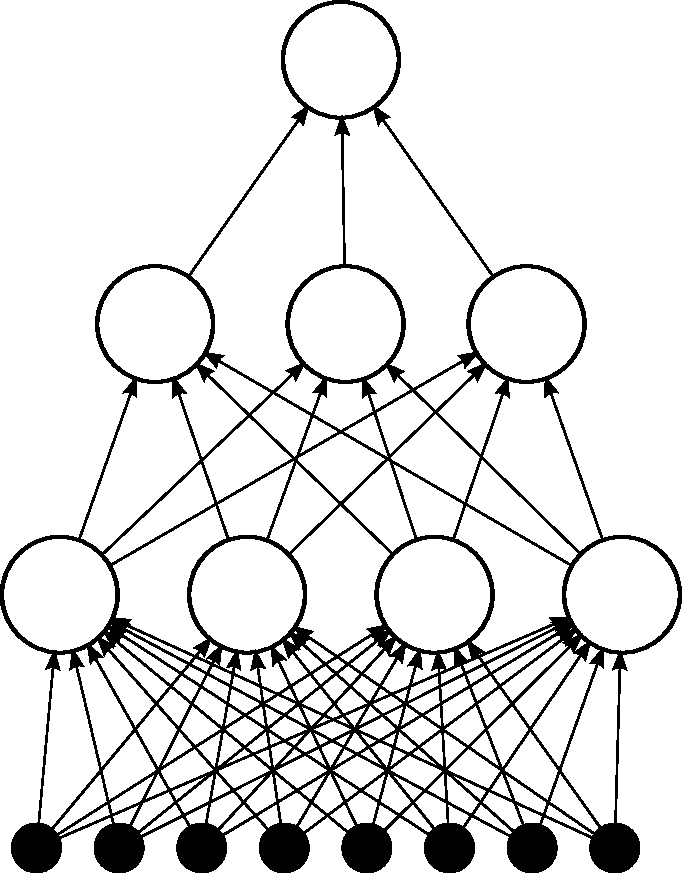
\includegraphics[width=0.3\textwidth]{images/ffnn}
  \end{center}
  \caption{Dopredná neurónová sieť}
  \label{fig:ffnn}
\end{figure}

\textbf{Viac vrstvová dopredná neurónová sieť} (obr. \ref{fig:ffnn}) je neurónová sieť zložená z viacerých vrstiev neurónov, pričom signál sa šíri len zo spodnejšej vrstve na vyššiu. V našej implementácii siete sa ako vstup každého neurónu berie výstup každého neurónu z predošlej vrstvy. Prvá vrstva dostane pôvodný vstup. 

Experimentami sme našli vhodné počty neurónov a vrstiev. Zvolili sme architektúru s 1 skrytou vrstvou s 45 neurónmi. V tabuľke \ref{tab:neuroncountcmp} je porovnanie úspešnosti na testovacích dátach a priemerná kvadratická chyba.

\begin{table}[hp]
\centering
\begin{tabular}{|l|l|c|c|}
\hline
\textbf{Vrstvy} & \textbf{Neuróny} & \textbf{Úspešnosť} & \textbf{Chyba}\\ \hline
2 & 40 & 81,11\% & 0,0818\\ \hline
2 & 45 & --\% & --\\ \hline
2 & 50 & 85,19\% & 0,0667\\ \hline
2 & 60 & 85,19\% & 0,0634\\ \hline
3 & 48; 12 & --\% & --\\
\hline
\end{tabular}
\caption{Porovnanie úspešnosti NS pri rôznych architektúrach}
\label{tab:neuroncountcmp}
\end{table}


\section{Viac vrstvová dopredná neurónová sieť - upravená verzia}

\begin{figure}[hp]
  \begin{center}
    \includegraphics[width=0.3\textwidth]{images/dffnn}
  \end{center}
  \caption{Upravená dopredná neurónová sieť}
  \label{fig:dffnn}
\end{figure}


V upravenej verzii sme upravili spodnú vrstvu siete - tú, ktorá dostáva vstup. Vstup je rozdelený na 16 častí a ku každej časti je pridelených niekoľko neurónov. Každý neurón spracúva len vstupy z jeho časti (obr. \ref{fig:dffnn}). 

Jej výhodou je rýchlosť. Náš vstup má rozmer $128\times 128 = 16384$, čo nie je malé číslo. Rozdelíme ho na 16 častí s veľkosťou $32\times 32 = 1024$. Takto namiesto toho aby každý vstupný neurón počítal s 16384 vstupmi počíta len s 1024, čo je $16\times$ rýchlejšie. Skupina neurónou pridelená danej časti sa stará len o príznaky zo svojej časti a nie je ovplyvňovaná ostatnými časťami. 

Nevýhodou je to, že neuróny sú fixne pridelené na jednotlivé vstupy. V pôvodnej sieti si neuróny sami vyberali, ktoré časti vstupu sú pre nich najvýznamnejšie a mohli tak lepšie pokryť vstup.

\begin{table}[hp]
\centering
\begin{tabular}{|l|c|c|}
\hline
\textbf{Neuróny} & \textbf{Úspešnosť} & \textbf{Chyba}\\ \hline
48; 12 & 83,33\% & 0,0745\\ \hline
112; 12 & --\% & --\\
\hline
\end{tabular}
\caption{Porovnanie úspešnosti NS pri rôznych architektúrach}
\label{tab:neuroncountcmp2}
\end{table}

%TODO
Keď si porovnáme tabuľku \ref{tab:neuroncountcmp2} s tabuľkou \ref{tab:neuroncountcmp} zistíme, že rozdiel v 

\section{Rekurentná neurónová sieť}